\documentclass[a4paper,class=article,border=10pt,tikz]{standalone}

%mypackages
\usepackage{pythontex}
\usepackage{pgfplots}
\usepackage{amsmath}
\usepackage{titlesec}
\usepackage{tikz}
\usetikzlibrary{shapes.geometric}
\usetikzlibrary{positioning}
\usetikzlibrary{snakes,calc,positioning,patterns,angles,quotes,decorations.pathmorphing,decorations.markings}
% \titleformat{<command>}[<shape>]{<format>}{<label>}{<sep>}{<before-code>}[<after-code>]
%\titleformat{\section}{\normalfont\Large\bfseries}{\thesection.}{10pt}{}
% \titlespacing{<command>}{<left>}{<before-sep>}{<after-sep>}
%\titlespacing{\section}{0pt}{14pt}{7pt}

%\titleformat{\subsection}{\normalfont\itshape}{\thesubsection.}{10pt}{}
%\titlespacing{\subsection}{0pt}{12pt}{6pt}
% set font encoding for PDFLaTeX, XeLaTeX, or LuaTeX
\usepackage{ifxetex,ifluatex}
\if\ifxetex T\else\ifluatex T\else F\fi\fi T%
  \usepackage{fontspec}
\else
  \usepackage[T1]{fontenc}
  \usepackage[utf8]{inputenc}
  \usepackage{lmodern}
\fi

\usepackage{hyperref}


\title{Title of Document}
\author{Name of Author}

% Enable SageTeX to run SageMath code right inside this LaTeX file.
% http://doc.sagemath.org/html/en/tutorial/sagetex.html
% \usepackage{sagetex}

% Enable PythonTeX to run Python – https://ctan.org/pkg/pythontex
% \usepackage{pythontex}

\begin{document}

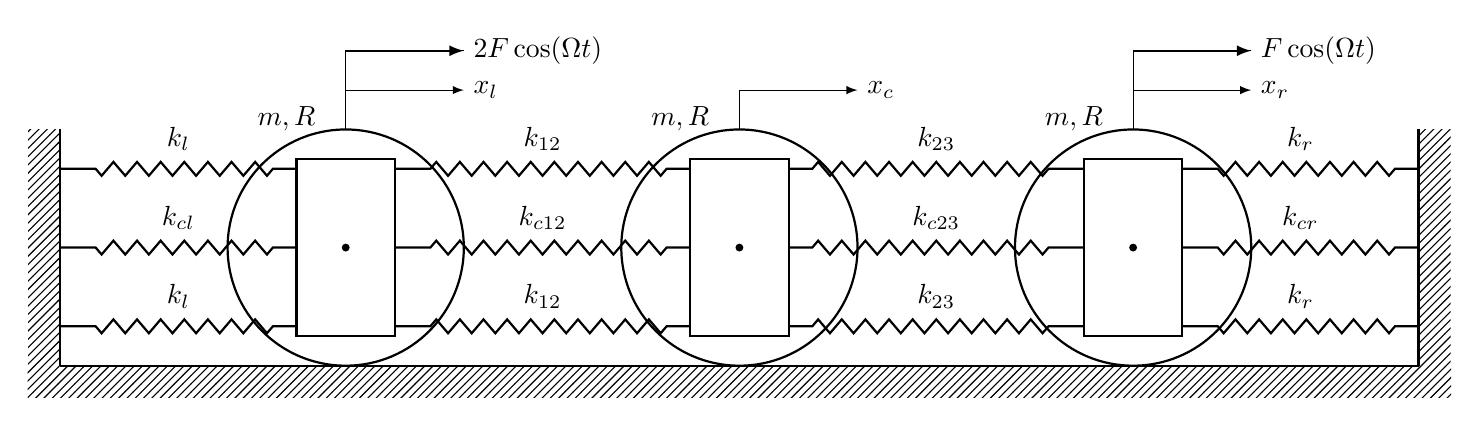
\begin{tikzpicture}
\tikzstyle{spring}=[thick,decorate,decoration={zigzag,pre length=0.3cm,post length=0.3cm,segment length=0.3cm}]
\tikzstyle{damper}=[thick,decoration={markings,  
  mark connection node=dmp,
  mark=at position 0.5 with 
  {
    \node (dmp) [thick,inner sep=0pt,transform shape,rotate=-90,minimum width=15pt,minimum height=3pt,draw=none] {};
    \draw [thick] ($(dmp.north east)+(2pt,0)$) -- (dmp.south east) -- (dmp.south west) -- ($(dmp.north west)+(2pt,0)$);
    \draw [thick] ($(dmp.north)+(0,-5pt)$) -- ($(dmp.north)+(0,5pt)$);
  }
}, decorate]
\tikzstyle{ground}=[fill,pattern=north east lines,draw=none,minimum width=0.75cm,minimum height=0.3cm]

\node (M) [draw,outer sep=0pt,thick,minimum width=1.25cm, minimum height=2.250cm,label={[yshift=-1.1cm]above:{}}] {};
\node (M2) [draw,outer sep=0pt,thick,minimum width=1.25cm, minimum height=2.250cm,xshift=5cm,label={[yshift=-1.1cm]above:{}}] at (M) {};
\node (M3) [draw,outer sep=0pt,thick,minimum width=1.25cm, minimum height=2.250cm,xshift=5cm,label={[yshift=-1.1cm]above:{}}] at (M2) {};

\node (Roller1) at (M) [draw,circle,outer sep=0pt,thick,minimum width=1.5cm, minimum height=3cm,label={[xshift=0.8cm, yshift=0.3cm]above left:{$m,R$}}] {};
\node (Roller2) at (M2) [draw,circle,outer sep=0pt,thick,minimum width=1.5cm, minimum height=3cm,label={[xshift=0.8cm, yshift=0.3cm]above left:{$m,R$}}] {};
\node (Roller3) at (M3) [draw,circle,outer sep=0pt,thick,minimum width=1.5cm, minimum height=3cm,label={[xshift=0.8cm, yshift=0.3cm]above left:{$m,R$}}] {};

%\node (ground) [ground,anchor=north west,xshift=-2.4cm,yshift=-0.25cm,minimum width=17.75cm] at (M.south west) {};
\node (wall_1) [ground,anchor=east,xshift=-3cm,yshift=0cm,minimum height=3.0cm ,minimum width=0.4cm] at (M.west) {};
\node (wall_2) [ground,anchor=west,xshift=3cm,yshift=0cm,minimum height=3.0cm ,minimum width=0.4cm] at (M3.east) {};

\draw[thick] (wall_1.south east) -- (wall_2.south west);
\draw[thick] (wall_1.north east) -- (wall_1.south east);
\draw[thick] (wall_2.north west) -- (wall_2.south west);
\draw[ground] (wall_2.south east)++(0,-0.4cm)  rectangle (wall_1.south west);


% \draw [thick] (M.south west) ++ (0.4cm,-0.125cm) circle (0.125cm)  (M.south east) ++ (-0.4cm,-0.125cm) circle (0.125cm);
% \draw [thick] (M2.south west) ++ (0.4cm,-0.125cm) circle (0.125cm)  (M2.south east) ++ (-0.4cm,-0.125cm) circle (0.125cm);
% \draw [thick] (M3.south west) ++ (0.4cm,-0.125cm) circle (0.125cm)  (M3.south east) ++ (-0.4cm,-0.125cm) circle (0.125cm);


\draw [spring]  (M2.180) ++ (0cm,0cm) -- ($ (M.0 )+(0cm,0cm)  $)  node [pos=0.5,above=0.10cm] (k_c12) {$k_{c12}$};
%\draw [fill=black]  (M2.180) ++ (0cm,0.15cm) rectangle ($ (M.0 )+(0cm,-0.15cm)  $) ;

\draw [spring]  (M2.0) ++ (0cm,0cm) -- ($ (M3.180 )+(0cm,0cm)  $)  node [pos=0.5,above=0.10cm] (k_c23) {$k_{c23}$};
%\draw [fill=black]  (M2.0) ++ (0cm,0.15cm) rectangle ($ (M3.180 )+(0cm,-0.15cm)  $) ;

\draw [spring]  (M.180) ++ (0cm,-0.0cm) -- ($ (wall_1.0 )+(0cm,0.0cm)  $) node [pos=0.5,above=0.10cm](k_cl) {$k_{cl}$};
%\draw [fill=black]  (M.180) ++ (0cm,0.15cm) rectangle ($ (wall_1.0 )+(0cm,-0.15cm)  $) ;

\draw [spring]  (wall_2.180) ++ (0cm,0cm) -- ($ (M3.0 )+(0cm,0cm)  $)node [pos=0.5,above=0.10cm] (k_cr) {$k_{cr}$};
%\draw [fill=black]  (wall_2.180) ++ (0cm,0.15cm) rectangle ($ (M2.0 )+(0cm,-0.15cm)  $) ;



\draw [spring]  (M2.180) ++ (0cm,1cm) -- ($ (M.0 )+(0cm,1cm)  $)  node [pos=0.5,above=0.10cm] (k_c12) {$k_{12}$};
\draw [spring]  (M2.0) ++ (0cm,1cm) -- ($ (M3.180 )+(0cm,1cm)  $)  node [pos=0.5,above=0.10cm] (k_c23) {$k_{23}$};

\draw [spring]  (M.180) ++ (0cm,1cm) -- ($ (wall_1.0 )+(0cm,1cm)  $) node [pos=0.5,above=0.10cm](k_l) {$k_l$};
\draw [spring]  (wall_2.180) ++ (0cm,1cm) -- ($ (M3.0 )+(0cm,1cm)  $)node [pos=0.5,above=0.10cm] (k_r) {$k_r$};


\draw [spring]  (M2.180) ++ (0cm,-1cm) -- ($ (M.0 )+(0cm,-1cm)  $)  node [pos=0.5,above=0.10cm] (k_c) {$k_{12}$};
\draw [spring]  (M2.0) ++ (0cm,-1cm) -- ($ (M3.180 )+(0cm,-1cm)  $)  node [pos=0.5,above=0.10cm] (k_c23) {$k_{23}$};
\draw [spring]  (M.180) ++ (0cm,-1cm) -- ($ (wall_1.0 )+(0cm,-1cm)  $) node [pos=0.5,above=0.10cm](k_l) {$k_l$};
\draw [spring]  (wall_2.180) ++ (0cm,-1cm) -- ($ (M3.0 )+(0cm,-1cm)  $)node [pos=0.5,above=0.10cm] (k_r) {$k_r$};


\draw [-latex,thin] (Roller1.north) --++ (0cm,0.5cm) -- +(1.5cm,0cm) node[right] {$x_l$};
\draw [-latex,thin] (Roller2.north) --++ (0cm,0.5cm) -- +(1.5cm,0cm) node[right] {$x_c$};
\draw [-latex,thin] (Roller3.north) --++ (0cm,0.5cm) -- +(1.5cm,0cm) node[right] {$x_r$};


\draw [thin] (Roller1.north) --++ (0cm,1cm) node (f_l_start) {}  --+ (1.5cm,0cm) node[right] (f_l_end) {$2F \cos(\Omega t)$};
\draw [-latex,thick]  (f_l_start.center)  --(f_l_end.west);

\draw [thin] (Roller3.north) --++ (0cm,1cm) node (f_p_start) {} --+  (1.5cm,0cm) node[right] (f_p_end) {$F \cos(\Omega t)$};
\draw [-latex,thick]  (f_p_start.center)  -- (f_p_end.west);

\fill[black] (M) circle (0.05);
\fill[black] (M2) circle (0.05);
\fill[black] (M3) circle (0.05);

\end{tikzpicture}
\end{document}